% ****************************************************************************************************
\chapter{Introduction}\label{ch:intro}
% ****************************************************************************************************

\section{Motivation}

\begin{itemize}
	\item "Understand the key elements and mechanisms in a specific business domain, as well as their relationships (Osterwalder \& Pigneur, 2002)", \citep[p. 303]{Pateli2004}
	\item "focuses on describing the elements and relationships that outline how a company creates and markets value", \citep[p. 7]{Osterwalder2005}
	\item "Modern business models are increasingly complex, particularly those with strong ICT and ebusiness components. The relationship between the different elements of a business model and the decisive success factors are not always immediately observable. Therefore the process of modelling social systems and, in this case, business models help identify and understand the relevant elements in a specific domain and the relationships among them [Morecroft 1994; Ushold and King 1995]. In addition, the visual representation of a business model usually enhances understanding.", \citep[p. 14]{Osterwalder2005}
	\item "As simple as this framework may seem, its power lies in the complex interdependencies of its parts. Major changes to any of these four elements affect the others and the whole. Successful businesses devise a more or less stable system in which these elements bond to one another in consistent and complementary ways.", \citep[p. 53]{Johnson2008}
	\item "A useful way to represent business models is by means of a causal loop diagram, where choices and consequences are linked by arrows based on causality theories" \citep[p. 198]{Casadesus-Masanell2010}
\end{itemize}


\section{Research Objectives}

Classify PaaS providers' business models and its main components. Reveal crucial interdependencies within PaaS business models using the concept of system dynamics resp. business dynamics.

\noindent Research Question(s):

\noindent How to design Platform as a Service business models in order to achieve a high adoption rate?
\begin{enumerate}
	\item How can business models of Platform as a Service providers' be classified?
	\item How are the Platform as a Service business model elements -- especially in regards to the platform adoption -- interrelated?
\end{enumerate}

\section{Research Methodology and Structure}

Design Science Research:
\begin{itemize}
	\item \citet{March1995}
	\item \citet{Hevner2004}
	\item \citet{Hevner2007}
	\item \citet{Peffers2007}
\end{itemize}

\begin{figure}[htb]
	\centering
	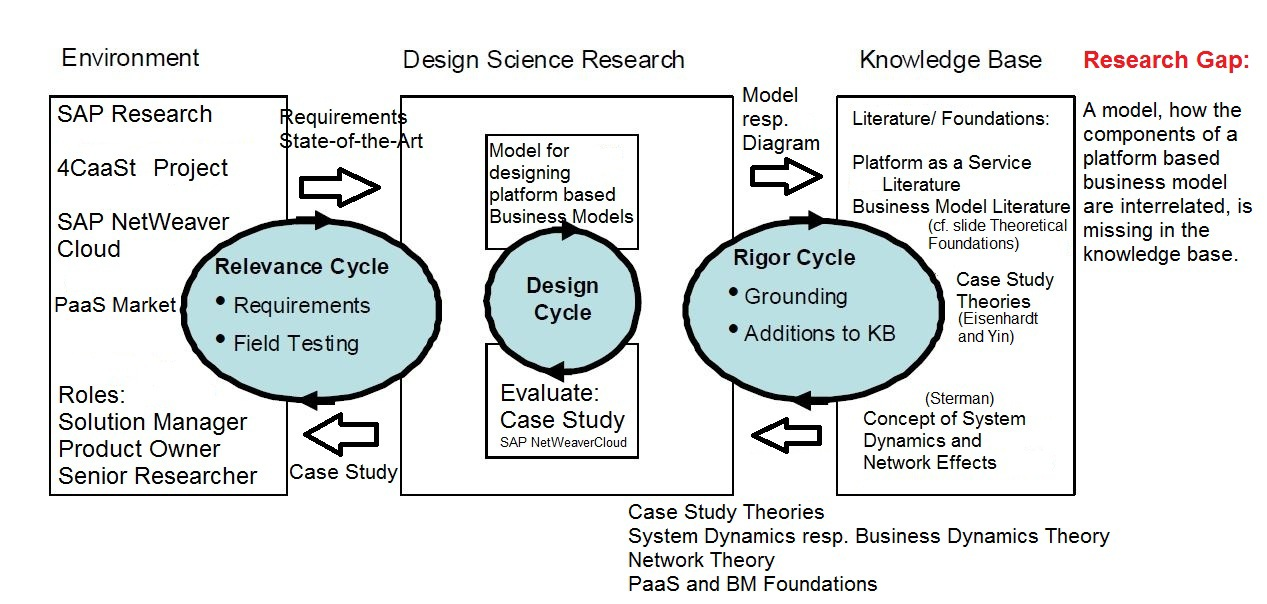
\includegraphics[width=\textwidth]{gfx/researchMethodology}
	\caption[Research Methodology]{Research Methodology adapted from \citet{Hevner2007}}
	\label{fig:rm}
\end{figure}